%
% File emnlp2016.tex
%

\documentclass[11pt,letterpaper]{article}
% \usepackage{emnlp2016}
\usepackage[accepted]{icml2013}
\usepackage{times}
\usepackage{latexsym}
\usepackage{lipsum}
\usepackage{graphicx}
% \usepackage{subfig}
\graphicspath{ {figures/} }
\usepackage{wrapfig, framed}
% \usepackage{natbib}
\usepackage{amsfonts}
\usepackage{amsmath} 
\usepackage{hyperref}
\usepackage{multirow,booktabs}
\usepackage{array}


% \usepackage[left=0.75in, right=0.75in]{geometry}


\newcommand\tab[1][1cm]{\hspace*{#1}}
\DeclareMathOperator*{\argmax}{\arg\!\max}
\newcolumntype{M}[1]{>{\centering\arraybackslash}m{#1}}

% TODO
% \title{Image Classification Via Selective Convex Combination of Semantics Embeddings}
\icmltitlerunning{Image Classification Via Selective Convex Combination of Semantics Embeddings}

% original-style author
% \author{Kritkorn Karntikoon \quad Korrawat Pruegsanusak \quad Suchan Vivatsethachai \\
% \{kritkorn, korrawat, suchanv\}@mit.edu}

\date{}

\begin{document}

\twocolumn[
\icmltitle{Image Classification Via Selective \\Convex Combination of Semantics Embeddings}

\icmlauthor{Kritkorn Karntikoon}{kritkorn@mit.edu}
\icmlauthor{Korrawat Pruegsanusak}{korrawat@mit.edu}
\icmlauthor{Suchan Vivatsethachai}{suchanv@mit.edu}

\vskip 0.4in
]
% \maketitle



\begin{abstract}
Image classification is one of the most classic classification that has been studied for a long time. While there are more and more image-label corpus, there are still a lots of images unseen or unlabeled. Giving that, it would be very beneficial if we could find a way to predict images which labels have been seen before. This is where zero-shot learning plays an important role. This paper particularly concentrates on the zero-shot learning that makes use of information from word embedding techniques in natural language processing. One of the paper, ConSE, proposes an ingenious way to get an information from word embedding space. However, we notice that there are still rooms to be improved in the original model. This paper will propose two models, which are based on ConSE, and provide insightful analysis on the performance of both models, using ConSE as a baseline.
\end{abstract}

% ==========================================
\section{Introduction}
One of the most challenging image classification tasks is $n$-way image label classification with low resource training data. Specifically, we want to predict a label of a particular image from the pool of $n$ labels the model has not seen before in the training. To achieve such prediction, we need to incorporate information from other sources. Such model is an example of a zero-shot learning, a model that predicts result in the space that it has not been trained before. ,

To infer information about the labels that the model has never seen,  we make use of word embedding space and relationship between embedding vectors. Several papers~\cite{devise, cvpr, cross-modal} have tried to connect relationship between image space and word embedding space to get a more robust prediction on an unseen image. 

One of the models, ConSE~\cite{conse}, use a simple but ingenious technique to connect two spaces together. They use CNN model trained on training data, testing images with label never seen in the training, and word embedding model which includes all the label from training and testing. For any given testing image, they first find top $t$ highest predicted labels from CNN. Those labels are from training dataset, so it is not the true label of the given image. They instead find a convex combination, which we call {\em synthetic} word embedding, of the word embeddings of those $t$ labels based on the predicted probability they get. Finally, the model will predict the label of which the word embedding has closest distance to the computed convex combination.  

In this paper, we try to improve upon zero shot learning introduced in ConSE~\cite{conse} to yield a better result. Instead of using naively constructed {\em synthetic} word embedding, we propose a revised {\em synthetic} word embedding which is constructed based on the synthetic vector itself. Specifically, in one proposed model, we get rid of some of the predicted labels that are "too far" from the original {\em synthetic} word embedding. In the other model, we get rid of the predicted labels that are "too similar" to labels that have higher probability. Doing so, we hope that we discover a model that are more insightful about the relationship of word embeddings, resulting in an increase of prediction accuracy. 

To get more insight about the important of convex combination of word embedding, we demonstrate the effect of the number of word embeddings ($T$) to be included in {\em synthetic} word embedding construction. We also explore the efficiency from different word embedding models with different embedding dimension and different size of corpus. This will give us some insight about how to choose word embedding model that allows zero-shot learning to yield a better result. Furthermore, to investigate the behavior of our proposed models deeper, we make the following observation:
\begin{itemize}
\item we look into some specific image that works better in our proposed model than in ConSE model, and demonstrate how it gets better. 
\item we show the performance of our proposed model on each different high-level category of testing images 
\end{itemize}

\subsection{Contributions}
Our main contribution is Threshold and Deviated model. Starting from ConSE Model, we create another step to remove outliers with respect to the synthetic vector, then we recompute and return the new result. We refer to this model as ``Threshold model."

After observing results from Threshold model, we propose another model by including labels that are substantially different from the synthetic vector, hoping that these labels contain information that will improve the model. This model is referred as ``Deviated model.''   

We also made our code available at
\url{https://github.com/korrawat/zeroshot}.

% ==========================================
\section{Problem Statement}
% Notations, ConSE (theoretical)
\tab We will present our model in a more mathematical rigorous way. $\mathcal{X}_0,\mathcal{X}_1$ be the set of all images in training dataset and testing dataset respectively, all with the same dimension and number of pixels. $\mathcal{Y}_0 = \{ \ell_1,\ell_2,...,\ell_a\}$ is the pool of all labels of the training images, while $\mathcal{Y}_1 = \{\ell_{a+1},...,\ell_{a+b} \}$ is the pool of all labels of the testing images. For each $i$, word label $\ell_i$ is English words describing the image. It is important to note that $\mathcal{Y}_0 \cap \mathcal{Y}_1 = \emptyset$. The training datasets consist of $(x_i,y_i)^{N}_{i=1}$ where $x_i \in \mathcal{X}_0$ and $y_i \in \mathcal{Y}_0$. Our goal is to predict the label of image $x' \in \mathcal{X}_1$ from the pool of labels $\mathcal{Y}_1 = \{\ell_{a+1},...,\ell_{a+b} \}$, which we have not seen before. This won't be possible unless we have connection between labels in $\mathcal{Y}_0$ and labels in $\mathcal{Y}_1$. Particularly, we incorporate a semantic word embedding function $\omega: \mathcal{Y}_0 \cup \mathcal{Y}_1 \rightarrow \mathcal{S}$ where $\mathcal{S}$ is a set of $q$-dimensional word embedding vector  $\{ s \mid s \in  \mathbb{R}^q \}$.

% ==========================================
\section{Models}
\subsection{ConSE Model}
\begin{figure*}[ht]\label{fig:pipeline}
\centering
{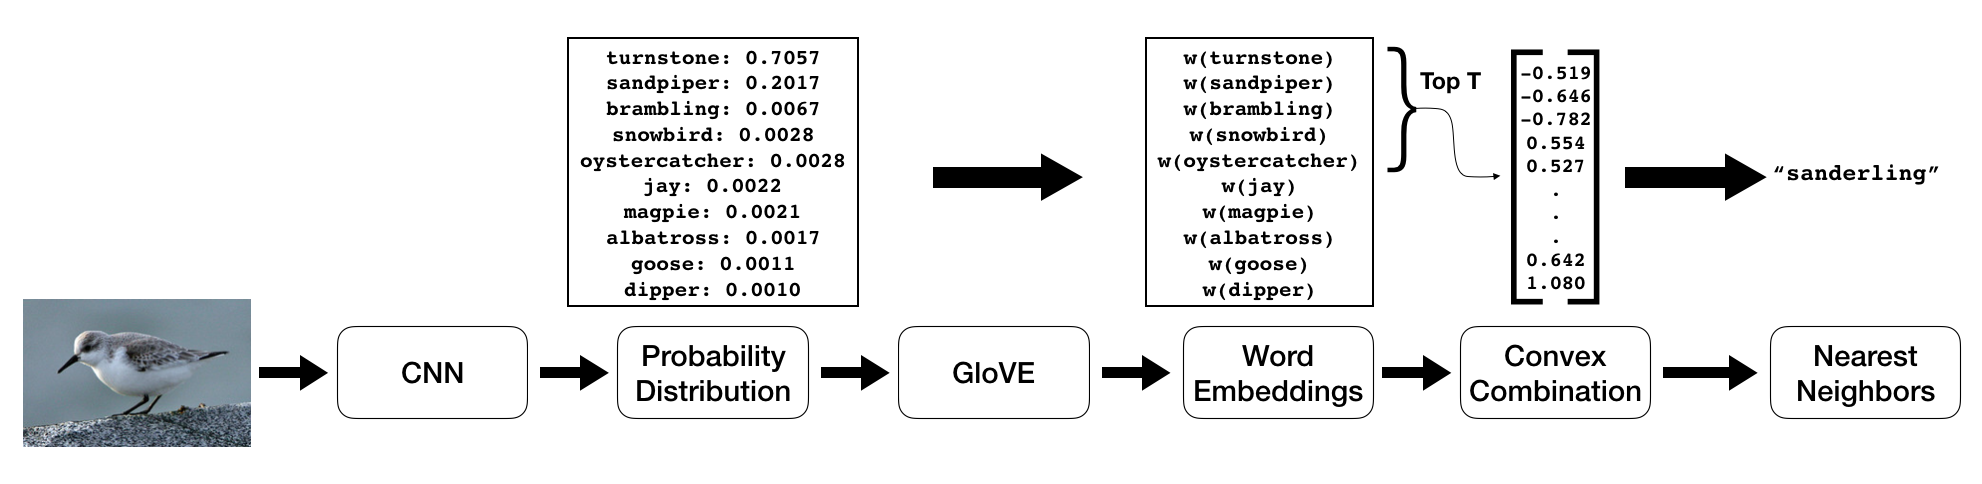
\includegraphics[width=1.8\columnwidth]{pipeline.png}}
\caption{
Procedure of ConSE Model. The input as a picture is parsed into the model. The model then uses CNN to compute the probability distribution of categories that are similar to the input. Then, we convert each category into word embedding and compute its weighted average. Finally, we return the label that is nearest to this average.
}
\end{figure*}

ConSE proposes the following model as shown in Figure \ref{fig:pipeline}. First, they use CNN model trained on $(x_i,y_i)^{N}_{i=1}$. Using this CNN model on testing image $x'$ gives a probability distribution $(p_1,p_2,...,p_m)$ corresponded to the training labels $(\ell_1,\ell_2,...,\ell_m)$. Lastly, they find a convex combination (a synthetic vector) of the first $T$ highest probability labels based on their predicted probability. Let $p(x',t)$ be the $t^{th}$ highest probability among $(p_1,p_2,...,p_m)$ and $\ell(x',t)$ be the corresponding label. We use only $T$ highest probability label to construct a synthetic word embedding
\begin{align*}
syn(x') = \sum\limits_{t = 1}^T \tilde{p}(x',t) \omega(\ell(x',t))
\end{align*}
where  $\tilde{p}(x',t)  = p(x',t) / \sum\nolimits_{t'=1}^T p(x',t') $, a normalized probability. Finally, they predict label 
\begin{align*}
\ell^* = \argmax_{\ell \in \mathcal{Y}_1} d(syn(x'), \ell)
\end{align*}
when $d(u,v)$ is a cosine similarity between vector $u$ and $v$

\subsection{Threshold Model}
\begin{figure}[ht]
        \centering
        \begin{frame}        {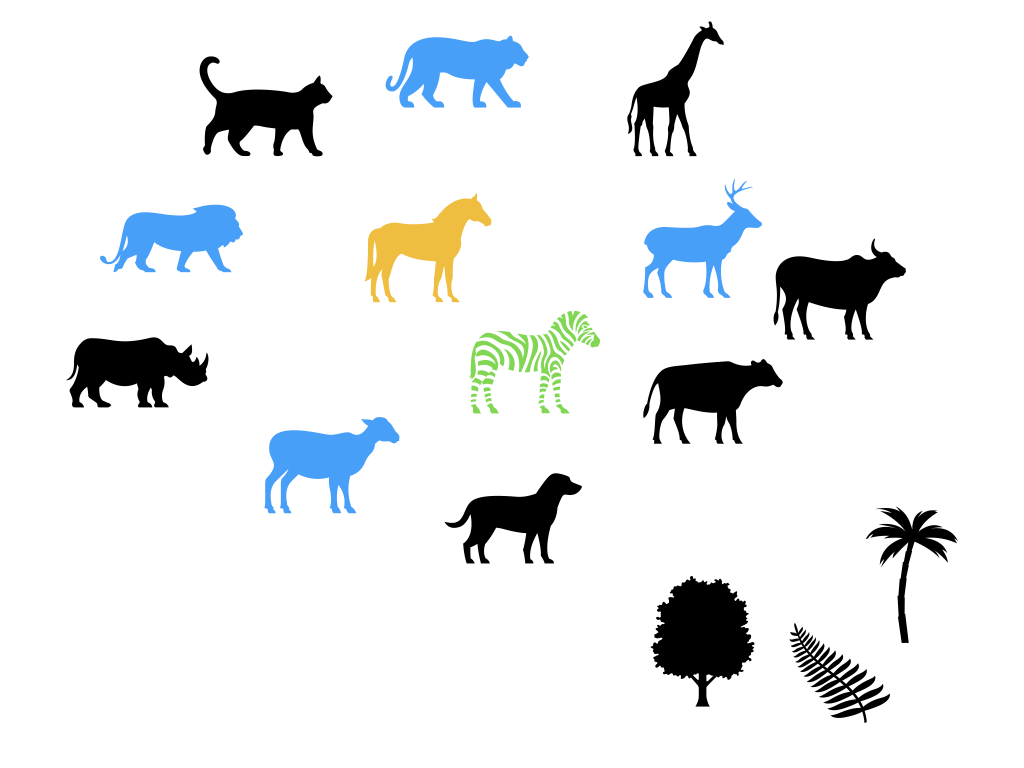
\includegraphics[width=0.48\columnwidth]{thm01.png}}
        \end{frame}\hfill
        \begin{frame}
 {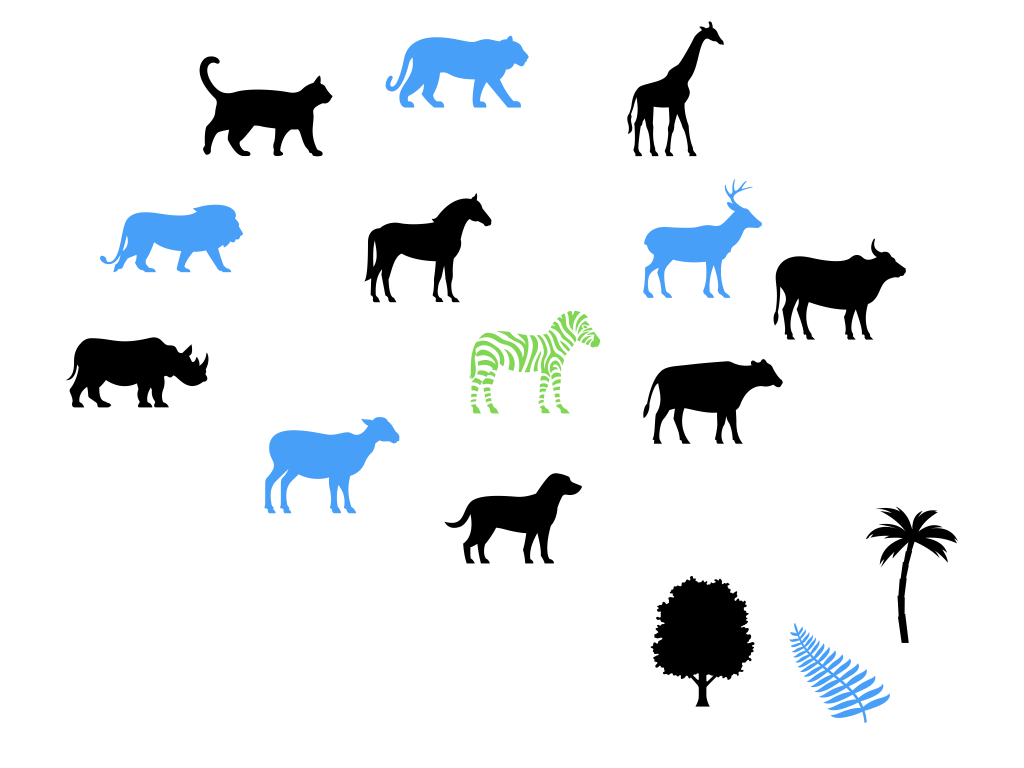
\includegraphics[width=0.48\columnwidth]{thm02.png}}
        \end{frame}
        \caption{Diagram illustrates the comparison between baseline and deviated model. The blue items represent the labels used to predict the result. The left hand side figure shows wrong predicted label (represented by yellow item) in the baseline model that can be improved by deviated model. The right hand side figure shows that deviated model will include substantial difference label and might lead to actual label (represented by green item)  
                \label{fig:thm}    
        }
\end{figure}

When we investigate the probability distribution from CNN for some image, we find that among the top $T$ highest probability, some are outrightly wrong. So instead of naively combining the top $T$ highest probability, we will screen some outlier out first. Specifically, for testing image $x' \in \mathcal{X}_1$, let the initial probability distribution from CNN be $(p_1,p_2,...,p_m)$. We first create a temporary synthetic vector 
\begin{align*}
tem  = \sum\limits_{t = 1}^T p(x',t) \omega(l(x',t))
\end{align*} 
, then we find a cosine similarity between $tem$ and each of $\omega(\ell_i)$ for $\ell_i \in \mathcal{Y}_0$. Let the resulting similarities be $(d_1,d_2,...,d_m)$ respectively. With threshold $\tau$, we screen out all label $\ell_i$ with $d_i < \tau$. We are left with label $(\ell'_1,\ell'_2,...,\ell'_{m'})$, with corresponding probability $(p'_1,p'_2,....,p'_{m'})$. Again, we define $p'(x',t)$ and $\ell'(x',t)$ be the $t^{th}$ highest probability among $(p'_1,p'_2,....,p'_{m'})$. Finally, we compute the final synthetic word embedding.
\subsection{Deviated Model}\label{model:deviated}
We also have another assumption that a substantial different labels need to contribute to the construction of a good {\em synthetic} word embedding. However, some of those labels may get too small probability that they are not included in the top highest $T$ probability. We propose a new model that allows labels, which have low probability but contains crucial information, to take part in the resulted {\em synthetic} word embedding as seen in Figure \ref{fig:thm}. Assume here that we still want the {\em synthetic} word embedding to be constructed from exactly $T$ word embeddings. Let $T = 2r$. First, we include the $r$ highest probability labels. Then for the next $2r$ highest probability labels, we will choose only $r$ to be included in the construction. We make selection based on the distance from the temporary word embedding constructed with only the first $r$ labels. Particularly, we first construct 
\begin{align*}
tem(x') = \sum\limits_{t=i}^r p(x',t)\omega(\ell(x',t)).
\end{align*}
Then we find a cosine similarity between $tem(x')$ and each of $\omega(\ell)$ for $\ell \in \{ \ell(x',r+1), \ell(x',r+2),...,\ell(x',3r) \}$ to get $d_{r+1},d_{r+2},...,d_{3r}$ respectively. Let $d'_{r+1}, d'_{r+2},...,d'_{3r}$ be sorted increasing order with corresponding labels $\ell'(x',r+1), \ell'(x',r+2), ..., \ell'(x',3r)$ and corresponding probability $p'(x',r+1), p'(x',r+2), ..., p'(x',3r)$, and . We then include the labels $\ell'(x',r+1), \ell'(x',r+2),..., \ell'(x,2r)$  in {\em synthetic} word embedding construction. In other words, we include only labels that are {\em more different } from the first $r$ labels so that the {\em synthetic} word embedding can gain extra information. The final word embedding is 
\begin{align*}
&syn(x') = \\
& \frac{1}{M} \left( \sum\limits_{t=1}^r p(x',t)\omega(\ell(x',t)) + \sum\limits_{t=r+1}^{2r} p'(x',t)\omega(\ell'(x',t)) \right)
\end{align*}
when $M$ is a normalized factor: $M = \sum_{t=1}^r p(x',t) + \sum_{t=r+1}^{2r} p'(x',t)$.

\section{Implementation Details}
% Maybe this deserves its own section?
% Subsection: CNN, Word vectors, ImageNet, Platform
Our models can be used with any Convolutional Neural Network architecture and any set of word vector representations. The CNN of our choice is the famous GoogLeNet~\cite{inceptionv1}, which was the winner of ImageNet Large-Scale Visual Recognition Challenge 2014 (ILSVRC 2014) with the top-5 classification error of 6.67\%. Even though there have been some researches that improve on the original GoogLeNet in the past few years, we think that this is a proper model for our project as it balances between performance and running time. While more recent models perform better on the regular image classification task, some need much more computational resources and it is not evident that they would perform better for our zero-shot image classification task. 

The word embeddings we choose is Global Vectors for Word Representation, or GloVe~\cite{pennington2014glove}. As opposed to other word embedding models, GloVe provides several word embeddings that are pre-trained with different sizes of text corpus and different dimension of vector representations.\footnote{Pre-trained GloVe is available at \url{https://nlp.stanford.edu/projects/glove}.} This allows us to explore the effects of these parameters on the performance.

The training and testing data is taken from ImageNet~\cite{imagenet_cvpr09}, an image database organized according to the WordNet tree (a hierarchy semantic tree). Each class of images is called a synset, with which is described by multiple labels associated. We call those labels describing each synset a ``synset's description''. It is important to note that some labels are not unigram, and some synset's description only contains label that is not unigram. However, since most word embedding models are trained on a bag of unigram words, we will only consider synset, which description contains at least one unigram label. We do so because practically we don't want to retrain word embedding every time we encounter new bigram label. This is essentially different from ConSE's implementation that retrains their word embedding with a new bag of words that include bigram labels from the training and testing synsets.

We use the CNN that is pre-trained with ILSVRC 2012 image classification dataset, which has $a = 1000$ labels\footnote{Pre-trained CNN in TensorFlow is available at \url{https://github.com/tensorflow/models/tree/master/research/slim}.}. For convenience, we will refer to this as the ``$1$K synsets''. For each synset in 1K synset, we choose only one unigram label from its description to represent the entire synset. This label will be the label that get converted to word embedding when we are constructing {\em synthetic} word embedding.

For testing synsets, we choose only those that are semantically close to the $1$K synsets. Specifically, we choose only synsets in WordNet tree that are within $2$ steps away from each synset in 1K synsets. Note that we must not include the synset in the training 1K synsets. We refer to these testing synsets as ``$2$-hops'' synsets. Lastly, to balance the testing images, we only include $200$ images from each of the synsets in $2$-hops. We disregard any synsets contain less than $200$ images. We end up with $295200$ testing images consisting of $1476$ final synsets, each of which contains $200$ images. The data can be downloaded from\footnote{The data can be downloaded from \url{http://www.image-net.org/}.}

We implement mostly everything in Python. We also use Amazon Web Services to get an access to GPU and multiple CPUs used to run the implementation.


% ==========================================
\section{Results}

We present the performances of our models with several sets of parameters. First, we introduce the evaluation metric and its calculation steps. Then, we compare the results of the baseline model (ConSE), the Threshold Model, and the Deviated Model. Lastly, we analyze the model performances by word categories.

\subsection{Evaluation Metric}
In this subsection, we analyze the performances of our models which is measured by following steps
\begin{enumerate}
\item For each image, find if the true label is in the top $k$ predictions
\item Count how many images is in each class get the correct label in top $k$ predictions, then divide that by number of images in the class
\item Average the metric for chosen classes
\end{enumerate}
This result will be referred in this paper as ``Hit@$k$''.

\subsection{Effects of word embeddings on the performance}
We explore how using different word embeddings affects the performance of the baseline ConSE model. 

From Table \ref{tab:wordemb}, we can see that as the dimension is increasing, the performance is better. This is quite different from what we expected before we did the experiment. At first, we expected that if the dimension is large, the word embedding space will be sparse. So, the predicted word embedding vectors will have less chance to encounter with any word in the space and so is the correct word as well. 

However, when we sample some words that give good accuracies, we can see that the sparsity of large dimensional word embedding spaces will also separate two unrelated words further (the distance is computed by cosine similarity). So, the chance that predicted word embedding vectors will choose wrong words given that it is predicted in the correct region will also decrease. %TODO: Toey wrote this for Milestone 5. James thinks it's still confusing.

Since the ``840B 300d'' version of GloVe provides the best performance, the results presented in subsequent sections will be based on this set of word vectors. We choose this to be the \textbf{baseline model}, because when starting with higher accuracy, we should be able to observe larger change when we adjust other parameters.

\begin{table}[t]
\caption{Effects of word embeddings on performance of the baseline model}
\label{tab:wordemb}
\begin{center}
\begin{small}
\begin{tabular}{cccccc}
\toprule
\multirow{2}{*}{Model} & \multicolumn{5}{c}{Precision hit@$k$ (\%)} \\
\cmidrule(lr){2-6}
& 1 & 2 & 5 & 10 & 20 \\
\midrule
6B 50d    & 3.8 & 5.6 & 9.2 & 13.3 & 18.5  \\
6B 100d   & 4.3 & 6.6 & 10.6 & 15.0 & 20.7  \\
6B 300d   & 5.4 & 8.3 & 13.9 & 19.6 & 26.5  \\
42B 300d  & 5.7 & 8.8 & 14.5 & 20.4 & 27.4  \\
840B 300d & 6.8 & 10.7 & 18.3 & 25.9 & 34.5  \\
\bottomrule
\end{tabular}
\end{small}
\end{center}
\end{table}

\subsection{Importance of convex combination}
We vary $T$, the number of CNN predictions to perform convex combination, and observe the performance. From Figure \ref{fig:tt}, we can see that using $T \geq 2$ significantly improves the performance over just $T = 1$ for both top-1 and top-10 predictions. This indicates the importance of using convex combination, as opposed to only using the top prediction from the CNN to find the nearest neighbors in word embedding space. 

However, as we increase $T$ from 6, the top-10 hit rate for the baseline model no longer improves, and the top-1 hit rate even starts to decline. This shows that while using more than one prediction to find a convex combination of word vectors is helpful, combining too many word vectors may be ineffective. This may be because the CNN predictions with lower probabilities include irrelevant words, thus deviating the synthetic vector away from the true label. This experiment inspire us to find other models that select only some of the top $T$ CNN predictions to combine into the synthetic vector.

\begin{figure}[ht]
\centering
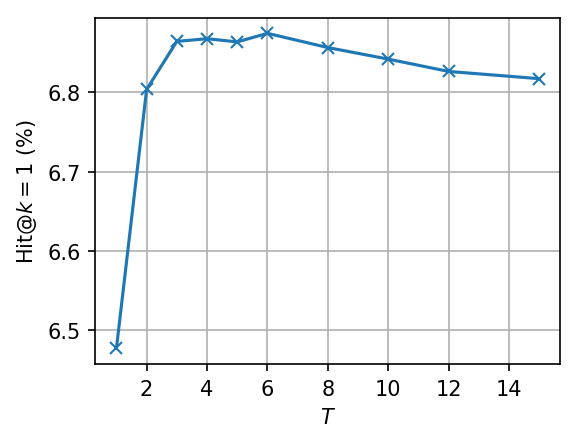
\includegraphics[width=0.48\columnwidth]{effect_tt_k1.png} \hfill
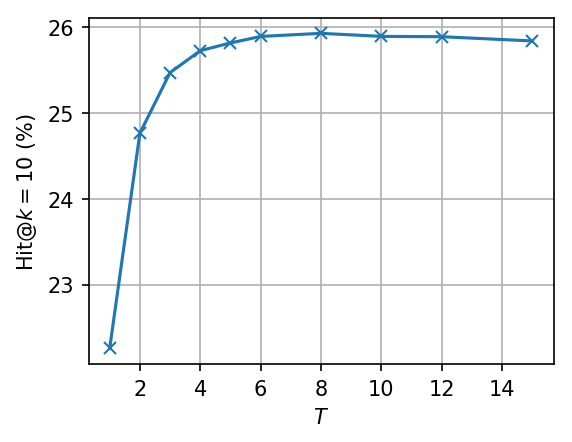
\includegraphics[width=0.48\columnwidth]{effect_tt_k10.png} 
\caption{Effects of $T$ on the performance of the baseline model.}
\label{fig:tt}
\end{figure}

% We conduct an experiment to validate the use of convex combination in ConSE by trying various values of $T$. 

% We can see from Figure \ref{fig:tt} that the actual word embedding does not rely solely on the label that has the most probability. As the value of $T$ is increasing, an accuracy of the baseline model is also increasing. This occurrence is due to the importance of other labels that have small probability but strong influence in terms of meaning. Thus, it is reasonable to use convex combination with the same weights as probability distribution to predict the word embedding of actual label.

\subsection{Threshold Model}
Since the similarity score is cosine, $\tau$ can vary from $-1.0$ to $1.0$. We do not consider the case when $\tau$ is too high ($\tau>0.6$ in practice), because this will most likely not reduce the number of involved labels anymore. 
% In fact, the highest NNs cosine similarity that we empirically observe is about 0.8

From Figure \ref{fig:threshold}, we can see that as the value of threshold is increasing, the Hit rate seems to remain unchanged until one point, at $\tau = 0.2$, where it drops significantly. One suspect is that when $t$ is large, the algorithm starts to remove the essential label from being used and result in an inaccurate prediction from partial components. In general, we can conclude that adjusting threshold will not significantly improve our model performance because the baseline ConSE model is equivalent to $\tau = -1.0$.

However, we empirically observe some examples as shown in Table \ref{tab:example} and see that there is an improvement in rank of actual label. As shown in \textit{shoe} example, the threshold, $t = 0.0$, removes ``shoe shop'' and ``plane'' which are not related to ``shoe'' in terms of meaning.   



% Hit plots
\begin{figure}[ht]
\centering
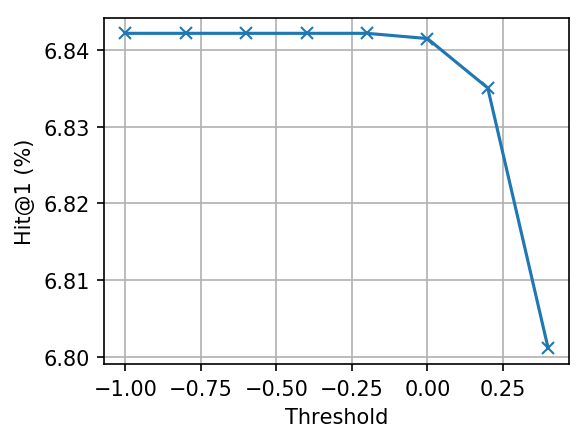
\includegraphics[width=0.48\columnwidth]{threshold_synbase_k1.png} \hfill
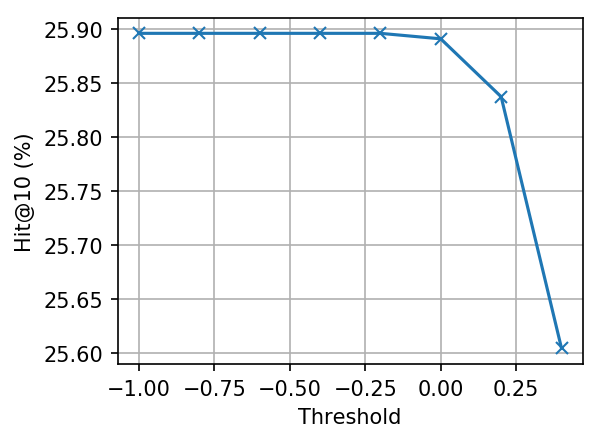
\includegraphics[width=0.48\columnwidth]{threshold_synbase_k10.png} 
\caption{Effects of threshold $\tau$ on the performance of the baseline model.}
\label{fig:threshold}
\end{figure}

\subsection{Deviated Model}
We experiment on the values of $r$ on the model described in Section \ref{model:deviated}, and compare its performance with base line model. Note that $r$ is equal to $T/2$ here. Figure \ref{fig:m3plot} shows the improvement of the deviated model (indicated in orange line) as the values of $r$ is increasing. However, when we observe Hit@1 and Hit@5 separately, we can see that Hit rate when $k=1$ improves significantly more and starts to drop as $r \geq 2$. Contrastingly, the Hit rate $k = 5$ for this deviated model is similar to the baseline and getting better than later as $r \geq 4$.    

We deduce that our model has a greater impact on predicting top 1 label than top 5 which is reasonable because the deviated model should theoretically benefit the testing image that relies greatly on the information from multiple training labels. As mentioned in \ref{fig:m3plot}, we aim to improve the performance by involving substantial difference labels. This will allow the model to improve the prediction marginally and give a small change in ranking the prediction. 

\begin{figure}[ht]
\centering
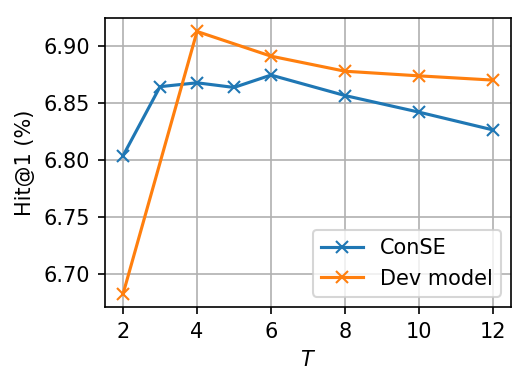
\includegraphics[width=0.48\columnwidth]{model3_k1.png} \hfill
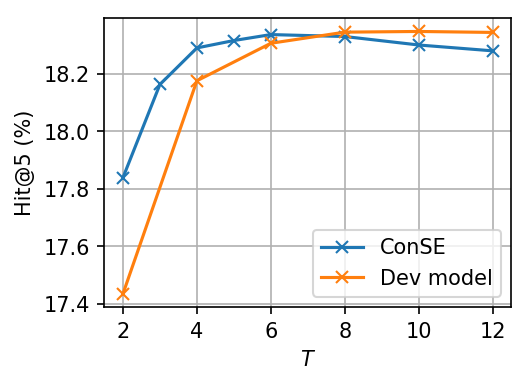
\includegraphics[width=0.48\columnwidth]{model3_k5.png} 
\caption{Comparison of hit rate of deviated model and the baseline model.}
\label{fig:m3plot}
\end{figure}

\subsection{Other Observations}

We observe that the variations between each model are relatively small. One question that may arise is whether the change in each model only affects the predictions of a few images, while leaving the rest unaffected. If this were the case, the effects of each model variation would be uninteresting and ineffective.

Therefore, we further analyze the words by high-level category to investigate what word categories perform well or badly. We can see from Table \ref{tab:category} that the deviated model mostly increases the prediction accuracy. Most of the categories benefits from the model, indicating that various and substantially different images get affected by our proposed model.

% analysis: animal names are specific (proper nouns)
% normal things are more ambiguous
% harder to train word embeddings with common words that have more than one different meanings, e.g. ``nest'', ``date'', ``hurdle''

\begin{table}[ht]
\caption{Hit@5 by word category. 840B 300d. A: ConSE, B: threshold $\tau = 0.2$, C: $r=5.$}
\label{tab:category}
\centering
\begin{small}
\begin{tabular}{M{9.5em}cccc}
\toprule
\multirow{2}{*}{High-level category} & \multirow{2}{*}{\shortstack{No. of\\ synsets}} & \multicolumn{3}{c}{Average hit@5 (\%)} \\
\cmidrule(lr){3-5}
& & A & B & C \\
\midrule
artifact, artefact & 999  & 16.96  & 16.89  & 17.02   \\
\addlinespace[0.5em]
animal, animate being, beast, brute, creature, fauna & 257  & 27.76  & 27.77  & 27.79   \\
\addlinespace[0.5em]
miscellaneous & 108  & 12.71  & 12.67  & 12.62   \\
\addlinespace[0.5em]
natural object & 56  & 8.91  & 8.93  & 8.85   \\
\addlinespace[0.5em]
geological formation, formation & 20  & 21.85  & 21.93  & 22.07   \\
\addlinespace[0.5em]
plant, flora, plant life & 19  & 6.08  & 6.00  & 6.21   \\
\addlinespace[0.5em]
fungus & 9  & 48.22  & 48.28  & 48.22   \\
\addlinespace[0.5em]
person, individual, someone, somebody, mortal, soul & 8  & 9.75  & 9.62  & 9.75   \\
\addlinespace[0.5em]
\midrule
Total & 1476 & 18.30  & 18.26  & 18.35  \\
\bottomrule
\end{tabular}
\end{small}
\end{table}


While the change in average hit is relatively small, the model affects many predictions. For example,
the number of images whose true labels were not in top-5 ConSE predictions but in top-5 model B predictions is 203, and the opposite is 330. 
For model C, the numbers are 1443 and 1304, respectively.
We can see that the recombination schemes of models B and C actually affect a lot of predictions. However, since the number of images whose predictions get better and those whose predictions get worse are approximately the same, the changes in average hit are relatively little. An interesting point here is how to eliminate the negatively affected predictions while keeping or increasing the number of improved predictions.

% \section{Discussion}
% Maybe put "Other Observations" here?
% Are the variations that we see too small to conclude anything?
% What else can we try (~future works) e.g. other CNN models, other Word Embeddings, other filtering scheme?
% precision: training and testing data are not drawn from the same distribution
% more examples 1) images per class 2) more classes, like hop 3 or all ImageNet data -- the further away the class is from the original prediction, the worse the performance is expected to be.
% (maybe should not mention?) repeated labels? 

\section{Conclusion}
% avoid using specific terms, should not present new data
% should be understandable without reading other sections of the report
We have investigated the zero-shot approach to $n$-way image classification model using convex combination of word embeddings. 
Using large database of images, we experimented and analyzed the direct approach, which simply combines the word vectors of top predictions from a Convolutional Neural Network, then find top nearest neighbors of this synthetic vector in the word embedding space.
Then we have proposed two variations of this baseline model, each of which employs a criterion to choose only some of the top predictions to recalculate the synthetic vector.
While one model barely benefits the prediction accuracy, the other model, which is based on the idea that different word embeddings all play an important role, increases the prediction accuracy by a little. Along with the analysis on the number of word embeddings we take into account in the baseline model, most of the results point to the direction that convex combination of word embedding indeed benefit the image classification task.

\section*{Division of Labor}
Three group members contributed equally. However, each of us focused on different sections of the project.
K.K. processed the image data from ImageNet, mainly implemented the threshold model and analysed the results
K.P. ran CNN and generated the plots for the report
S.V. focused on the processing word embeddings, introduced the new deviated model, and analyzed its results.

\section*{Acknowledgments}
We would like to thank the instructors of Machine Learning class (6.867) Professor Devavrat Shah, Assistant Professor David Sontag, Professor Suvrit Sra and our TA Curtis Northcutt for giving helpful advice and feedback during the development of our project.


\bibliography{cit}
% \bibliography{citation}
% \bibliographystyle{icml2013}
\bibliographystyle{plain}
% \bibliographystyle{emnlp2016}


%%%%%%%%%%%%%%%%%%%%%%%%%%%%%%%%%%%%%%%%%%%%%%%%%%
% Example tables
%%%%%%%%%%%%%%%%%%%%%%%%%%%%%%%%%%%%%%%%%%%%%%%%%%
\begin{table*}[t]
\caption{Examples of our models, based on 840B 300d word embeddings. Blue refers to selected labels in threshold $\tau=0.0$ model, and pink refers to selected labels in the $r=3$ Deviated Model. ``Sim'' refers to the cosine similarity between each word label and the first synthetic vector.}
\label{tab:example}
\begin{center}
\begin{small}
\resizebox{\textwidth}{!}{\begin{tabular}{clrrll}
\toprule
\multirow{2}{*}{Image}
& \multicolumn{3}{c}{Softmax over 1K synsets}
& \multicolumn{1}{c}{ConSE}
& \multicolumn{1}{c}{Our Threshold Model ($\tau=0.0$)} \\
\cmidrule(lr){2-4}
\cmidrule(lr){5-5}
\cmidrule(lr){6-6}
& \multicolumn{1}{c}{Labels}
& \multicolumn{1}{c}{Prob}
& \multicolumn{1}{c}{Sim}
& \multicolumn{1}{c}{Labels}
& \multicolumn{1}{c}{Labels} \\
\midrule

\multirow{10}{*}{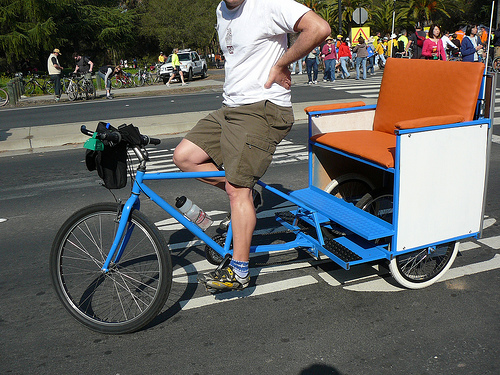
\includegraphics[height=10em]{n03904433_4368.JPEG}}
& \textcolor{blue}{bicycle-built-for-two, tandem bicycle, tandem} & $0.117$& $0.617$& scooter & \textbf{pedicab, cycle rickshaw} \\
& \textcolor{blue}{jinrikisha, ricksha, rickshaw} & $0.115$& $0.635$& water scooter, sea scooter, scooter & scooter \\
& \textcolor{blue}{tricycle, trike, velocipede} & $0.097$& $0.796$& \textbf{pedicab, cycle rickshaw} & water scooter, sea scooter, scooter \\
& \textcolor{blue}{unicycle, monocycle} & $0.047$& $0.642$& velocipede & velocipede \\
& \textcolor{blue}{barrow, garden cart, lawn cart, wheelbarrow} & $0.031$& $0.513$& parasail & parasail \\
& \textcolor{blue}{moped} & $0.027$& $0.578$& skateboard & skateboard \\
& \textcolor{black}{file, file cabinet, filing cabinet} & $0.013$& $-0.015$& toboggan & toboggan \\
& \textcolor{blue}{crate} & $0.010$& $0.252$& hearse & hearse \\
& \textcolor{blue}{carton} & $0.009$& $0.163$& luge & luge \\
& \textcolor{blue}{shopping cart} & $0.009$& $0.400$& kayak & kayak \\

\midrule

\multirow{10}{*}{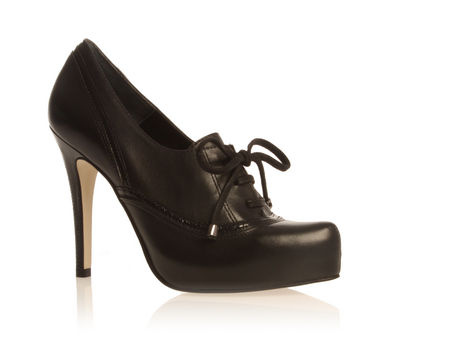
\includegraphics[height=10em]{n02904927_20825.JPEG}}
& \textcolor{blue}{Loafer} & $0.613$& $0.949$& moccasin, mocassin & moccasin, mocassin \\
& \textcolor{blue}{clog, geta, patten, sabot} & $0.167$& $0.523$& slingback, sling & slingback, sling \\
& \textcolor{blue}{sandal} & $0.115$& $0.650$& espadrille & espadrille \\
& \textcolor{blue}{cowboy boot} & $0.039$& $0.304$& brake shoe, shoe, skid & \textbf{brogan, brogue, clodhopper, work shoe} \\
& \textcolor{black}{shoe shop, shoe-shop, shoe store} & $0.016$& $-0.008$& shoe & brake shoe, shoe, skid \\
& \textcolor{blue}{holster} & $0.004$& $0.085$& \textbf{brogan, brogue, clodhopper, work shoe} & shoe \\
& \textcolor{blue}{running shoe} & $0.004$& $0.485$& chukka, chukka boot & chukka, chukka boot \\
& \textcolor{blue}{buckle} & $0.002$& $0.380$& bomber, grinder, hero, hero sandwich, ... & bomber, grinder, hero, hero sandwich, ... \\
& \textcolor{black}{plane, carpenter's plane, woodworking plane} & $0.001$& $-0.096$& blucher & blucher \\
& \textcolor{blue}{mailbag, postbag} & $0.001$& $0.069$& instep & instep \\

\midrule

\multirow{10}{*}{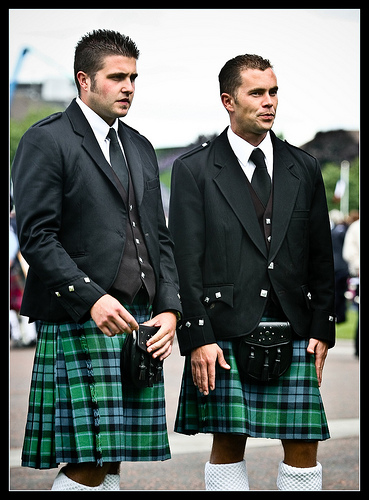
\includegraphics[height=10em]{n04395106_19387.JPEG}}
& \textcolor{blue}{suit, suit of clothes} & $0.729$& $0.986$& singlet, vest, undershirt & singlet, vest, undershirt \\
& \textcolor{blue}{miniskirt, mini} & $0.071$& $0.393$& slacks & slacks \\
& \textcolor{blue}{Windsor tie} & $0.037$& $0.448$& jump suit, jumpsuit & jump suit, jumpsuit \\
& \textcolor{blue}{trench coat} & $0.027$& $0.411$& \textbf{tartan, plaid} & gown, surgical gown, scrubs \\
& \textcolor{black}{Loafer} & $0.024$& $-0.020$& gown, surgical gown, scrubs & nightgown, gown, nightie, night-robe, ... \\
& \textcolor{blue}{groom, bridegroom} & $0.014$& $0.358$& nightgown, gown, nightie, night-robe, ... & \textbf{tartan, plaid} \\
& \textcolor{blue}{bow tie, bow-tie, bowtie} & $0.013$& $0.332$& suiting & suiting \\
& \textcolor{blue}{bolo tie, bolo, bola tie, bola} & $0.008$& $0.139$& trouser & trouser \\
& \textcolor{blue}{racket, racquet} & $0.003$& $0.206$& case, compositor's case, typesetter's case & case, compositor's case, typesetter's case \\
& \textcolor{blue}{lab coat, laboratory coat} & $0.003$& $0.481$& casing, case & casing, case \\

\midrule

\multirow{10}{*}{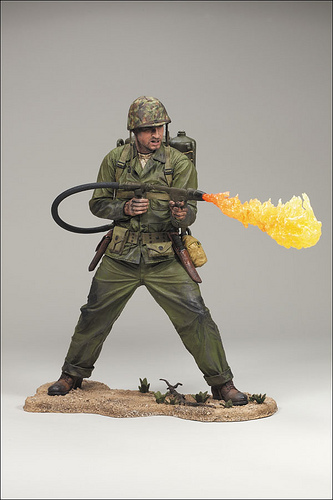
\includegraphics[height=10em]{n03356559_12703.JPEG}}
& \textcolor{magenta}{parachute, chute} & $0.166$& $0.739$& singlet, vest, undershirt& automatic pistol, automatic \\
& \textcolor{magenta}{assault rifle, assault gun} & $0.122$& $0.520$& automatic pistol, automatic& \textbf{flamethrower} \\
& \textcolor{black}{gasmask, respirator, gas helmet} & $0.087$& $0.490$& grease-gun, gun& singlet, vest, undershirt \\
& \textcolor{black}{military uniform} & $0.057$& $0.486$& goggles& drogue, drogue chute, drogue parachute \\
& \textcolor{black}{ski} & $0.057$& $0.432$& camouflage, camo& catapult, launcher \\
& \textcolor{magenta}{rifle} & $0.050$& $0.573$& camouflage& parasail \\
& \textcolor{magenta}{bulletproof vest} & $0.043$& $0.248$& cannon& blimp, sausage balloon, sausage \\
& \textcolor{magenta}{ballplayer, baseball player} & $0.029$& $0.208$& carbine& beret \\
& \textcolor{magenta}{pickelhaube} & $0.024$& $0.298$& \textbf{flamethrower}& turret \\
& \textcolor{black}{scuba diver} & $0.021$& $0.433$& revolving door, revolver& camouflage, camo \\

\midrule

\multirow{10}{*}{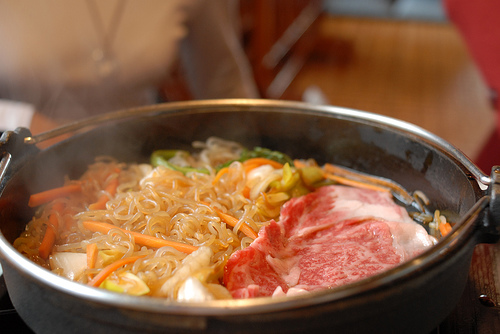
\includegraphics[height=10em]{n07879174_6939.JPEG}}
& \textcolor{magenta}{hot pot, hotpot} & $0.146$& $0.781$& crock, earthenware jar& \textbf{sukiyaki} \\
& \textcolor{magenta}{caldron, cauldron} & $0.074$& $0.622$& paella& petite marmite, minestrone, ... \\
& \textcolor{magenta}{wooden spoon} & $0.066$& $0.458$& petite marmite, minestrone, ...& jambalaya \\
& \textcolor{magenta}{wok} & $0.056$& $0.697$& colander, cullender& crock, earthenware jar \\
& \textcolor{black}{soup bowl} & $0.035$& $0.514$& jambalaya& tempura \\
& \textcolor{magenta}{spaghetti squash} & $0.028$& $0.485$& \textbf{sukiyaki}& paella \\
& \textcolor{black}{Crock Pot} & $0.026$& $0.600$& gravy& terrine \\
& \textcolor{magenta}{butternut squash} & $0.026$& $0.485$& risotto, Italian rice& gumbo \\
& \textcolor{black}{carbonara} & $0.022$& $0.529$& couscous& gumbo, okra \\
& \textcolor{black}{ladle} & $0.021$& $0.635$& tempura& croquette \\

\midrule


\multirow{10}{*}{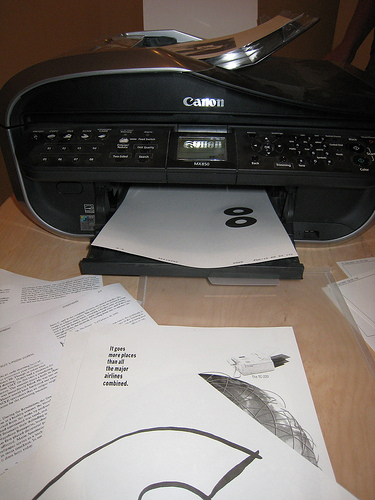
\includegraphics[height=10em]{n03316105_29720.JPEG}}
& \textcolor{magenta}{printer} & $0.370$& $0.909$& scanner, digital scanner, image scanner& scanner, digital scanner, image scanner \\
& \textcolor{black}{CD player} & $0.130$& $0.609$& toner& toner \\
& \textcolor{magenta}{projector} & $0.124$& $0.639$& background, desktop, screen background& background, desktop, screen background \\
& \textcolor{magenta}{modem} & $0.085$& $0.583$& \textbf{facsimile, facsimile machine, fax}& adapter, adaptor \\
& \textcolor{magenta}{mouse, computer mouse} & $0.080$& $0.473$& adapter, adaptor& print \\
& \textcolor{magenta}{photocopier} & $0.048$& $0.633$& print& router \\
& \textcolor{black}{tape player} & $0.038$& $0.609$& router& screen door, screen \\
& \textcolor{black}{cassette player} & $0.015$& $0.609$& screen door, screen& \textbf{facsimile, facsimile machine, fax} \\
& \textcolor{magenta}{desktop computer} & $0.011$& $0.409$& stylus, style& stylus, style \\
& \textcolor{black}{laptop, laptop computer} & $0.008$& $0.592$& flatcar, flatbed, flat& cable, cable television, cable system, ...\\


\bottomrule
\end{tabular}}
\end{small}
\end{center}
\end{table*}

\end{document}
